\documentclass[journal]{IEEEtran}
% Draft for IEEE Transactions on Cognitive and Developmental Systems (TCDS).
% Build: pdflatex main && bibtex main && pdflatex main && pdflatex main
% Storyline, evidence and references: ../paper_planning.md (the master planning document).
% TCDS limits: abstract 150-250 words; regular papers longer than 10 pages (references and biographies
% included, supplementary material excluded) pay an overlength charge, so this paper must end by page 10.
% supplement.tex holds the supplementary material (not counted).

\usepackage{amsmath,amssymb}
\usepackage{graphicx}
\usepackage{booktabs}
\usepackage{xcolor}
\usepackage{cite}
\usepackage{url}
\usepackage[hidelinks]{hyperref}

% ---------------------------------------------------------------- draft markers
% \draftmarkerstrue: working draft, with the red and blue markers and, after the biographies, a page
% listing the citations to be sourced. \draftmarkersfalse: submission version, without any of them.
\newif\ifdraftmarkers
\draftmarkerstrue
% \citeneeded{...}: a claim that needs a source outside the LM/npj reference lists.
% The text is a description of the kind of source needed, never an invented reference.
\makeatletter
\newcommand{\citeneeded}[1]{\ifdraftmarkers\textcolor{red}{[CITE:~#1]}\addtocontents{cnd}{\protect\item #1}\fi}
\newcommand{\listofcitationsneeded}{%
  \IfFileExists{\jobname.cnd}{\begin{enumerate}\setlength{\itemsep}{1pt}\small\@starttoc{cnd}\end{enumerate}}%
    {\@starttoc{cnd}(compile again to list them)}}
\makeatother
% \authornote{...}: a point for the authors to check before submission.
\newcommand{\authornote}[1]{\ifdraftmarkers\textcolor{blue}{\textit{[Authors: #1]}}\fi}

\newcommand{\eav}{\varepsilon_{Av}}
\newcommand{\eam}{\varepsilon_{Am}}
% placeholder photo for the biographies (1 in x 1.25 in, as in the final paper)
\newcommand{\photoplaceholder}{\fbox{\parbox[c][1.15in][c]{0.9in}{\centering\footnotesize\textcolor{gray}{photo}}}}

\begin{document}

\title{From Coupled to Estimation-Coupled Oscillators: Grounding Attachment Dynamics in a Robot Dyad}

\author{Aung~Htet,
        Alejandro~Jimenez-Rodriguez,
        Marcantonio~Gagliardi,
        and~Tony~J.~Prescott%
\thanks{A. Htet and A. Jimenez-Rodriguez are with the School of Computing and Digital Technologies, Sheffield Hallam University, UK (e-mail: aung.htet@student.shu.ac.uk; a.jimenez-rodriguez@shu.ac.uk). A. Htet and A. Jimenez-Rodriguez contributed equally.}%
\thanks{M. Gagliardi is with the Institute for Lifecourse Development, University of Greenwich, UK (e-mail: m.gagliardi@greenwich.ac.uk).}%
\thanks{T. J. Prescott is with the Department of Computer Science, The University of Sheffield, UK (e-mail: t.j.prescott@sheffield.ac.uk).}%
\thanks{This article extends a conference paper presented at Living Machines 2024~\cite{Htet2024}; Section~\ref{sec:intro} sets out the relation between the two. Supplementary material is available online.}}

\markboth{IEEE Transactions on Cognitive and Developmental Systems --- draft}%
{Htet \MakeLowercase{\textit{et al.}}: From Coupled to Estimation-Coupled Oscillators}

\maketitle

\begin{abstract}
Robots that interact with people can couple their behaviour to a partner only through what they sense. We examine this requirement in a coupled-oscillator model of attachment, in which a child and a caregiver are motivational oscillators whose coupling terms, the physical and the emotional distance between them, are computed from both partners' internal needs and so are grounded in nothing either partner perceives. We first characterise what the coupling does: synchrony, anti-synchrony, an inhomogeneous steady state born in a saddle-node bifurcation, a shared exploratory state and irregular oscillation near the transitions. We then show that the regimes leave distinct signatures in distance and vocal exchange, in a simulated strange situation and with two physical MiRo robots. Networks trained on these signals estimate the coupling terms, which turns the model into oscillators coupled through estimation. In 577 validated runs of two simulated MiRo robots, robots whose partner models run on their own estimates lose coordination: each keeps believing in a coordinated relationship while the real needs drift apart, because the two models are detuned, and the synchrony seen from identical starts is an unstable symmetric state. Coordination returns only when the partner model follows a reference model and the robot perceives its partner, and the regimes can then be read from behaviour, with 89\% accuracy from both robots. Grounding the coupling requires anchored, not merely accurate, estimates.
\end{abstract}

\begin{IEEEkeywords}
Social robotics, coupled oscillators, attachment, grounding, partner models, coordination dynamics, strange situation.
\end{IEEEkeywords}

% =====================================================================
\section{Introduction}
\label{sec:intro}

\IEEEPARstart{R}{obots} are being built to keep people company over long periods, as companions at home, aids in care and partners in therapy~\cite{Prescott2021,Collins2013}, and the relationships people form with them can help or harm~\cite{Prescott2021,Sharkey2010}. To relate well, a robot must respond to a person's needs, but those needs are interoceptive, sensed only from within~\cite{Craig2002}. Whatever couples the robot's behaviour to the person's must therefore pass through what the robot senses, as in assistive systems that infer a user's affective state~\cite{Robillard2018} or in robots designed to entrain with a user's rhythms~\cite{Lomas2022resonance}. Models of interaction rarely meet this requirement: their coupling terms are usually written in terms of the partners' internal states. What does it take to ground them in perception?

Attachment is a natural test case, because it is the prototype of a relationship that both partners regulate through behaviour. Bowlby described child and mother as a system in dynamic equilibrium, in which each partner's attachment, care or exploration elicits or inhibits the other's and keeps the distance between them within limits~\cite{Bowlby1982}. The strange situation procedure (SSP) made this equilibrium observable~\cite{Ainsworth1978,Prince2021,Chow2018representing}, human bonds show biobehavioural synchrony~\cite{Feldman2017}, and individual differences vary along the dimensions of avoidance and ambivalence~\cite{Fraley2003infant,Gagliardi2021our}.

We previously modelled this system as two coupled motivational oscillators, a child that seeks care and a caregiver that provides it, with an attractive avoidance coupling and a repulsive ambivalence coupling~\cite{Htet2024,Dixit2019dynamics}. Following Gagliardi's distinction between physical availability and emotional bond~\cite{Gagliardi2022}, the coupling acts through two terms, a physical and an emotional distance. In the model, however, these terms are computed from both partners' needs: each agent reads the other's need, as in the closest agent-based account of the SSP~\cite{Gagliardi2022}, and the distances measured on the robots of~\cite{Htet2024} only modulated a coupling that still did so. The coupling was ungrounded. Bowlby's own account differs: each partner acts on a working model of the other, which becomes fitted to the partner only gradually~\cite{Bowlby1982} \authornote{page numbers in the 1982 edition}.

Here we ground the coupling in three steps (Fig.~\ref{fig:concept}). We characterise what the coupling does (Section~\ref{sec:model}). We show that its regimes leave signatures in the distance between the partners and in their vocal exchange, in a simulated SSP and with two physical robots (Section~\ref{sec:behaviour}). And we replace the coupling terms by estimates learned from those signals, so that each of two simulated MiRo robots~\cite{Prescott2017miro} carries a private working model of the dyad and is coupled to its partner only through estimation (Section~\ref{sec:private}). Two design factors define four such robots: the estimate is blind to the partner or perceives it, and the partner model follows the robot's own estimate or a reference model of the partner. We test them in 577 Gazebo runs, each checked against its controller, and offline from random starting needs.

The answer has five parts (Section~\ref{sec:results}). Coupled through the true coupling terms, the robots coordinate visibly. Coupled through their own estimates, each robot keeps believing in a coordinated relationship while the real needs drift apart, because the two models are detuned. Synchrony from identical starts is an unstable symmetric state. Coordination returns only with an anchored partner model, one that follows a reference model while the robot perceives its partner. And the regimes can then be read from behaviour.

The conference version~\cite{Htet2024} introduced the model, a first analysis of its regimes and a physical-robot demonstration with the coupling computed from both needs. The extended analysis, the behavioural signatures in simulation and on physical robots, the estimation-coupled robots and their tests are new. The supplementary material gives further detail (Sections~S1--S8).

\begin{figure*}[t]
\centering
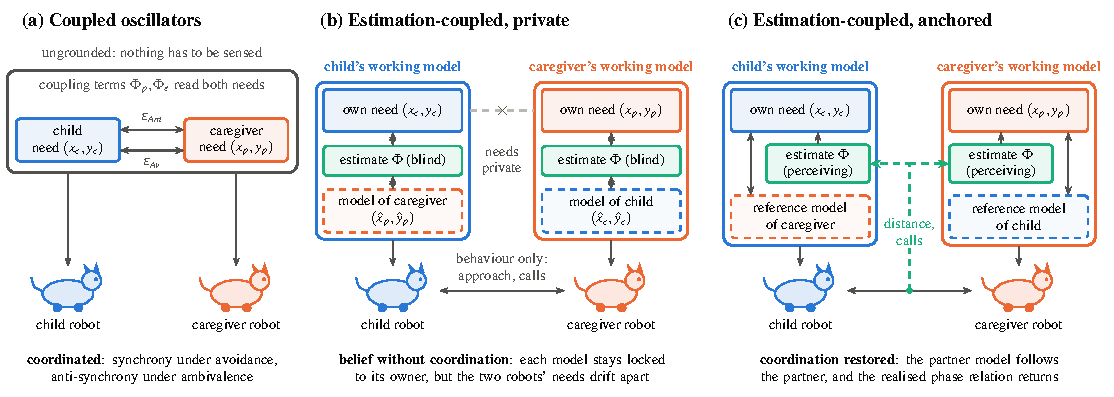
\includegraphics[width=\textwidth]{figures/fig_concept.pdf}
\caption{From coupled to estimation-coupled oscillators. (a) In the coupled model the coupling terms, attractive under avoidance ($\eav$) and repulsive under ambivalence ($\eam$), are computed from both needs. (b) Estimation-coupled robots each hold a copy of the dyad, with an estimate $\Phi$ of the coupling and a model of the partner (dashed), and interact only through behaviour. (c) In the anchored design the partner model follows a reference model of the partner and the estimate perceives the partner through distance and calls.}
\label{fig:concept}
\end{figure*}

% =====================================================================
\section{Background}
\label{sec:background}
Human--robot relationships are best understood relationally, by what each partner brings to the interaction~\cite{Prescott2021}. People form attachments to assistive technologies~\cite{Collins2013}, robots for children raise concerns about emotional harm~\cite{Sharkey2010}, and assistive systems increasingly model the user's state explicitly: BayesACT infers a user's affective identity and acts to keep the interaction aligned~\cite{Robillard2018}, and resonance, the rhythmic entrainment of partners, has been proposed as a design strategy for social robots~\cite{Lomas2022resonance}. Estimating a partner's state is a long-standing problem in social robotics \citeneeded{user-state estimation / theory of mind in social robotics}; how such an estimate shapes the joint dynamics of a pair is less studied.

Bowlby described attachment with the concepts of control theory: the child's attachment system has proximity to the caregiver as its set-goal and the caregiver's behaviour is organised likewise~\cite{Bowlby1982}. Ainsworth's SSP related infants' patterns to their mothers' responsiveness at home~\cite{Ainsworth1978}, taxometric analysis favours dimensions over categories~\cite{Fraley2003infant}, and Gagliardi links avoidance to the caregiver's emotional insensitivity, ambivalence to physical unresponsiveness and disorganisation to a third dimension~\cite{Gagliardi2021our,Gagliardi2022}. Computational models of attachment go back to Bowlby's own use of control systems~\cite{Petters2019attachment}: Stevens and Zhang modelled attachment as a homeostatic system with the caregiver's responsiveness as a parameter~\cite{Stevens2009dynamic}, mathematical models of the SSP treat the mother as a regulator of the child's anxiety~\cite{Buono2006}, and robots have been given imprinting-like bonds~\cite{Canamero2011}. Coupled oscillators describe partners' physiology~\cite{Helm2012coupled,Palumbo2016interpersonal}, attractive and repulsive coupling yield synchrony, anti-synchrony and oscillation death~\cite{Dixit2019dynamics}, a frequency difference lets the relative phase of coordinating partners wander~\cite{Kelso1995} \authornote{chapter of~\cite{Kelso1995}}, and pulse-coupled oscillators synchronise from almost any start~\cite{Mirollo1990}. All of these couple partners through their actual states.

% =====================================================================
\section{The Coupled-Oscillator Model and Its Regimes}
\label{sec:model}

Each agent $i\in\{c,p\}$, child or caregiver, has a need $x_i$, a fast motivational state that makes it approach its partner when $x_i>0$ and explore when $x_i<0$, and an accumulated need $y_i$. Following the attractor framework for motivational conflict~\cite{Jimenez2020framework,Prescott2025plm}, the need descends a double-well potential tilted by the accumulated need, and the accumulated needs are coupled:
\begin{align}
\dot{x}_i &= x_i - 2x_i^3 - y_i, \label{eq:fast}\\
\dot{y}_c &= \mu\,(b\,x_c - \eam\Phi_p - \eav\Phi_e), \nonumber\\
\dot{y}_p &= \mu\,(b\,x_p + \eam\Phi_p - \eav\Phi_e), \label{eq:slow}
\end{align}
with the physical and emotional distance terms
\begin{equation}
\Phi_p = \tfrac{1}{2}(y_c+y_p) + y_c,\qquad \Phi_e = k_0\big(\tfrac{1}{2}(y_c-y_p) + y_c - \delta\big),
\label{eq:phi}
\end{equation}
$b=0.5$, $k_0=0.8$, $\delta=0.1$ and $\mu=0.1$. Ambivalence enters the two agents with opposite signs and pushes their needs apart; avoidance enters both alike and draws them together~\cite{Dixit2019dynamics}. The fast--slow structure~\cite{Bertram2017} makes each uncoupled agent a relaxation oscillator. The distance terms, Eq.~\eqref{eq:phi}, are functions of both needs, which is what makes the coupling ungrounded.

What does the coupling do? We integrated the model along both strips and over the plane (Fig.~\ref{fig:canonical}; Section~S2). From random starts, weak ambivalence keeps the needs synchronised, with a median correlation of 0.90 at $\eam=0.1$. Stronger ambivalence desynchronises them, anti-synchronises them ($-0.96$ at $\eam=0.7$) and slows the oscillation, until it dies on an inhomogeneous steady state in which the child's need is fixed in approach and the caregiver's in exploration: an unavailable caregiver. This state is born in a saddle-node bifurcation at $\eam=b$, with $\bar{x}_c^2=(\eam-b)/(2\eam)$, but stays unstable until $\eam\approx0.75$; in between, oscillation persists with returns that vary from cycle to cycle. Under avoidance the needs are anti-synchronised at first ($-0.94$ at $\eav=0.1$) and synchronise as avoidance grows ($0.67$ at $\eav=0.6$), until both settle, from $\eav\approx0.69$, on a shared fixed point in exploration: an avoidant dyad. Over the plane (Fig.~\ref{fig:canonical}e), 81\% of the parameter pairs oscillate, 5\% settle and 14\% escape at strong combined coupling. Irregular oscillation, which does not lock to a fixed phase, appears in 10\% of the plane, near weak coupling and near the transitions; it is a candidate for the disorganised dimension of attachment~\cite{Gagliardi2021our}.

\begin{figure*}[t]
\centering
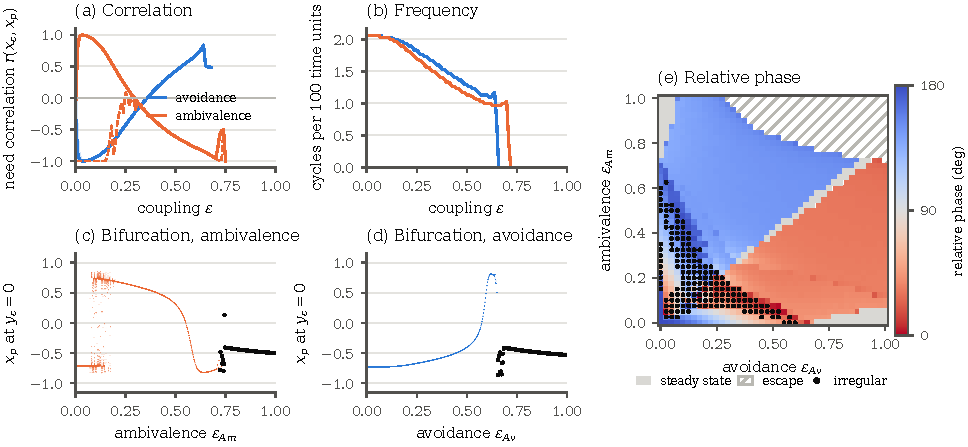
\includegraphics[width=\textwidth]{figures/fig_canonical.pdf}
\caption{Regimes of the coupled model, Eqs.~\eqref{eq:fast}--\eqref{eq:phi}. (a) Correlation of the needs along the two strips: median and interquartile range over 20 random starts (solid) and from an anti-synchronised start (dashed). (b) Frequency of the child's need. (c,d) Bifurcation diagrams: the caregiver's need where the child's accumulated need crosses zero upwards (coloured), and steady states (black). (e) Mean relative phase over the plane from an anti-synchronised start (0: in phase; 180: anti-phase), with steady states, escapes and irregular oscillation.}
\label{fig:canonical}
\end{figure*}

% =====================================================================
\section{Physical and Emotional Distance in Behaviour}
\label{sec:behaviour}

If the coupling terms are to be grounded, the regimes must be visible in what a partner can sense. We first ran the model in an agent-based SSP (Fig.~\ref{fig:sim}; Section~S3). Two point agents share a square room; the caregiver stays near a central base, the child explores the corners when its need is negative and returns to the base when it is positive, and both call while in approach and answer each other's calls. The physical distance is the Euclidean distance between the agents and emotional contact is the exchange of calls. The time the child spent near the caregiver separated the regimes: 50\% when secure, 38\% and 18\% under moderate and strong avoidance, and 53\% and 100\% under moderate and strong ambivalence ($\chi^2=14{,}676$, $N=50{,}000$). The calls separated them too: the strongly ambivalent child called through a third of the time while the caregiver stayed silent.

The same signatures appeared with two physical MiRo-e robots running the coupled model in a robot SSP, with the distance measured from the robots' positions and the calls produced by MiRo's vocal synthesiser~\cite{Moore2017biomimetic} (Section~S4). The secure child spent 54\% of the time near the caregiver, the strongly avoidant child 41\% and the moderately ambivalent child 43\% ($\chi^2=99.4$, $N=29{,}743$); the secure regime differed from the other two, and the ambivalent robot spent more time away than the simulation predicted. Distance and vocal exchange thus carry the regime, which makes them the signals in which to ground the coupling.

\begin{figure*}[t]
\centering
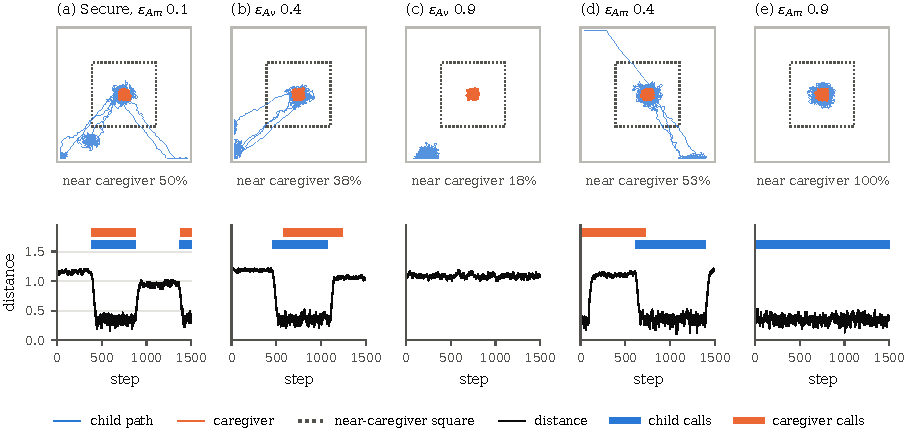
\includegraphics[width=\textwidth]{figures/fig_sim_ssp.pdf}
\caption{The regimes in a simulated SSP, at $(\eav,\eam)$ given above each panel. Top: the child's path (blue) over the last 3000 steps, the caregiver (orange) and the square of half the room's width around the base (dotted). Bottom: the distance between the agents and their calls over 1500 steps.}
\label{fig:sim}
\end{figure*}

% =====================================================================
\section{Estimation-Coupled Oscillators}
\label{sec:private}

\subsection{Learning the coupling terms from behaviour}
\label{sec:learned}
A robot cannot evaluate Eq.~\eqref{eq:phi}, because it does not know its partner's accumulated need. We trained networks, in the agent-based SSP of Section~\ref{sec:behaviour}, to estimate the coupling terms from signals a robot can sense:
\begin{equation}
\begin{aligned}
d_p^{(i)} &= \hat{\Phi}_p\big(s_i,\; x_i,\; y_i,\; \eam\big),\\
d_e^{(i)} &= \hat{\Phi}_e\big(\epsilon_i,\,v_{\bar{\imath}},\,v_i,\; x_i,\; y_i,\; \eav\big),
\end{aligned}
\label{eq:learned}
\end{equation}
where $s_i$ is a distance input, $v_i$ and $v_{\bar{\imath}}$ are the robot's own and its partner's calls, and $\epsilon_i$ is a trace of vocal evidence that grows when the partner answers (Section~S1). None of the inputs is the partner's need. The estimates are accurate offline: their median error is 0.028--0.041 for $\varepsilon\geq0.1$, the physical estimate rests mainly on the robot's own need, and the emotional estimate needs the calls (Section~S5).

\subsection{Private working models}
Each robot $i$ integrates its own copy of the dyad, $z^{(i)}=(x_c^{(i)},y_c^{(i)},x_p^{(i)},y_p^{(i)})$, and acts on its own component, the child on $x_c^{(c)}$ and the caregiver on $x_p^{(p)}$ (Fig.~\ref{fig:architecture}). The other half is its partner model, written $(\hat{x}_p,\hat{y}_p)$ for the child and $(\hat{x}_c,\hat{y}_c)$ for the caregiver: the self, the partner and their interaction that Bowlby ascribed to a working model~\cite{Bowlby1982}. The robot controllers write the coupling in the distance form of the robot implementation of~\cite{Htet2024},
\begin{equation}
\begin{aligned}
\dot{x}_i &= 2x_i - 4x_i^3 - y_i,\\
\dot{y}_c &= b'x_c - \eam\,(y_c + y_p - d_p) - \eav\,(y_p - y_c - d_e),\\
\dot{y}_p &= b'x_p - \eam\,(y_c + y_p + d_p) - \eav\,(y_p - y_c - d_e),
\end{aligned}
\label{eq:distance}
\end{equation}
with $b'=0.7$, integrated by RK4 at 30 control ticks per second. With $d_p,d_e$ set to the coupling terms of the true needs, the \emph{coupled reference}, Eq.~\eqref{eq:distance} synchronises under avoidance and anti-synchronises under ambivalence from weak coupling on, and its needs escape at strong coupling where the model of Section~\ref{sec:model} settles (Section~S2 compares the two).

\begin{figure}[t]
\centering
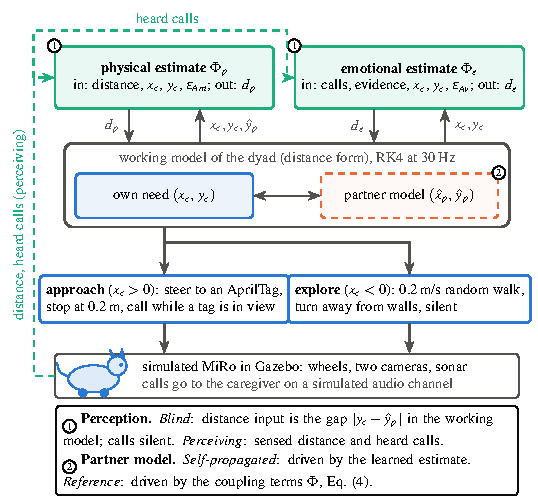
\includegraphics[width=\columnwidth]{figures/fig_architecture.pdf}
\caption{Controller of one robot (the child). Networks estimate the coupling terms $d_p$ and $d_e$ from the robot's own need and a distance and call input; the working model holds the robot's own need, which selects approach or exploration, and its model of the caregiver. The two design factors are marked (1) and (2). The caregiver's controller is the same; it stays on its box and calls while $x_p>0$.}
\label{fig:architecture}
\end{figure}

\subsection{Two design factors}
\label{sec:designs}
Two choices define how a robot's working model meets its partner. A \emph{blind} estimate is fed the gap $|y_c^{(i)}-y_p^{(i)}|$ inside the robot's own copy and silent calls; a \emph{perceiving} estimate is fed the sensed distance between the robots and the calls they actually make. A \emph{self-propagated} partner model is driven by the robot's own estimate; a \emph{reference} partner model is driven by the coupling terms evaluated on the robot's copy, so it follows the model of how the partner behaves. We call the perceiving design with a reference partner model \emph{anchored} and the blind, self-propagated design \emph{private models}. A perceiving robot without a partner model is a further control (Section~S5). If every copy used the true coupling terms, the copies would be identical and would reproduce the coupled reference; we verified this numerically. They differ because each robot's estimate is conditioned on its own need, which can shift each copy's frequency, and in the blind design, from identical starting needs under avoidance, the two halves of every copy stay equal, so a symmetric start can hide an instability.

% =====================================================================
\section{Methods}
\label{sec:method}

\emph{Offline analysis.} We integrated the controllers outside the robot software exactly as the robots do. Along each strip one parameter varied from 0 to 1 in steps of 0.02, from 40 random starting needs drawn from $U(-1,1)$ and from the identical start $(-1,1,-1,1)$ of~\cite{Htet2024}, over 54 model time units, the length of a 180~s robot run, and over 300 units with the first 100 discarded (\emph{after transients}). To test the stability of the identical start, we raised the caregiver's accumulated need by $10^{-9}$ to $10^{-1}$ and integrated for 2000~s.

\emph{Robots in Gazebo.} Two simulated MiRo robots~\cite{Prescott2017miro,Mitchinson2016miro} were placed in a $2.61\times2.61$~m arena under ROS \citeneeded{ROS and Gazebo} (Section~S6). The caregiver sits on a 0.3~m box carrying an AprilTag on each face \citeneeded{AprilTag fiducial detection}. When exploring, the child drives at a commanded 0.2~m/s with a random turn rate; when approaching, it steers to a tag and stops 0.2~m from the box. The child calls while approaching with a tag in view and the caregiver while its own need is in approach, on a simulated Boolean channel. Each controller logs its working model and estimates at every tick; positions come from ground truth.

\emph{Runs and validation.} We recorded 577 runs, most of them 180~s long (Section~S8). At each strip value private models were run from five random starts and the identical start, the coupled reference from three random starts and the identical start, and the other designs from three random starts. With blind estimates or the coupled reference the needs do not depend on behaviour, so replaying the controller from the logged start must reproduce them; it did in every run (correlation above 0.999). With perceiving estimates the logged inputs matched the recorded distance and calls.

\emph{Measures.} \emph{Coordination} is the correlation $r(x_c,x_p)$ between the robots' own needs, \emph{belief} the correlation $r(x_c,\hat{x}_p)$ inside the child's model, and \emph{partner tracking} the correlation $r(\hat{x}_p,x_p)$. \emph{Detuning} is the difference between two needs' frequencies (zero crossings over twice the duration). An estimate's accuracy is its correlation with the coupling terms of the true needs. \emph{Call reciprocity} is the fraction of the child's calling time with a caregiver call within 3~s. A run \emph{escapes} when a need exceeds 10 in magnitude. Offline results are medians over starts; Gazebo results are means with 95\% intervals over runs. Random forests \citeneeded{random forests} trained on 1110 runs of a kinematic stand-in classified runs as secure ($\varepsilon\leq0.1$), avoidant or ambivalent and estimated $(\eav,\eam)$ from the child's distance and calls, or also from the caregiver's calls, and were tested on 176 Gazebo runs of private models (Section~S7).

% =====================================================================
\section{Results}
\label{sec:results}

\subsection{The coupled reference: coordination the robots can show}
\label{sec:r1}
Coupled through the true coupling terms, the robots coordinate from any starting state. From random starts the needs synchronise under avoidance and anti-synchronise under ambivalence (grey in Fig.~\ref{fig:strips}a,b): over a 180~s run the median coordination is 0.94 at $\eav=0.2$ and $-0.98$ at $\eam=0.2$, and after transients it reaches $\pm1.00$ wherever the needs stay bounded. The robots agree, with mean coordination of $+0.94$ and $-0.95$. Under avoidance the caregiver calls whenever the child seeks it and answers every one of its calls (Fig.~\ref{fig:timelines}a); under ambivalence it calls while the child explores and falls silent when the child approaches, answering 0.29 of the calls at $\eam=0.2$ (Fig.~\ref{fig:timelines}c), the pattern of an unavailable caregiver. Coordination thus has a behavioural signature. Its limits are escapes, from $\eav=0.24$ and $\eam=0.44$ (Fig.~\ref{fig:strips}c,d).

\begin{figure*}[t]
\centering
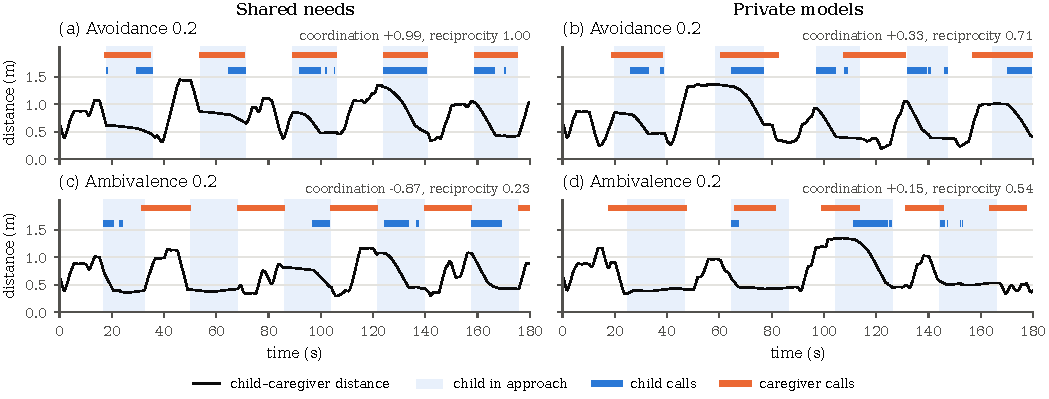
\includegraphics[width=\textwidth]{figures/fig_gazebo_timelines.pdf}
\caption{Gazebo runs of the coupled reference and of private models from the same random starting needs, at $\varepsilon=0.2$: distance between the robots, periods with the child in approach (shaded) and the calls of the child and the caregiver (bars), over the first 180~s.}
\label{fig:timelines}
\end{figure*}

\begin{figure*}[t]
\centering
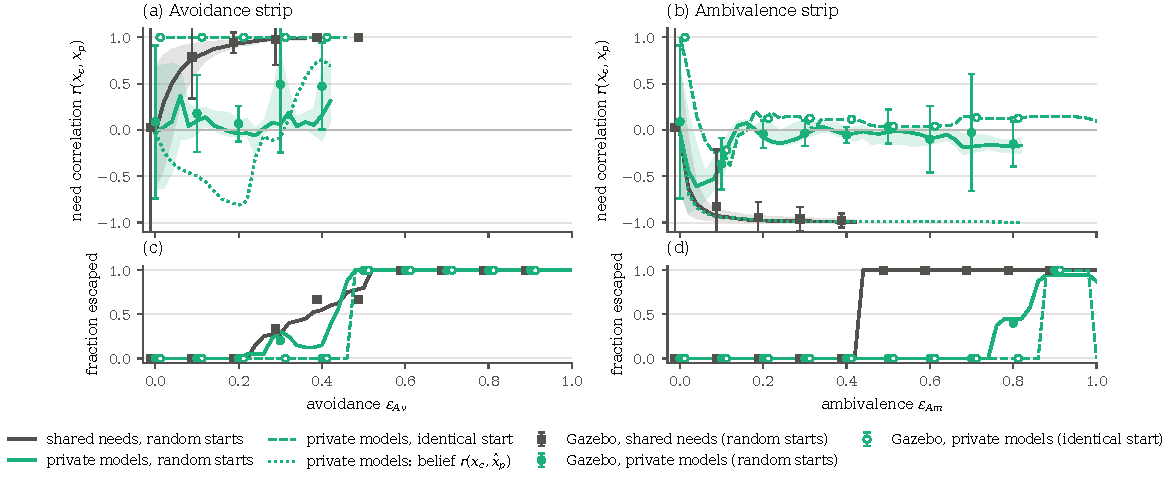
\includegraphics[width=\textwidth]{figures/fig_strips.pdf}
\caption{The coupled reference (``shared needs'', grey) and private models (green) along the two strips over a 180~s run. (a,b) Coordination: median and interquartile range over 40 random starts, private models from the identical start (dashed) and the child's belief with private models (dotted). Markers: Gazebo runs, mean and 95\% interval over seeds; runs that escaped are omitted. (c,d) Fraction of runs that escape.}
\label{fig:strips}
\end{figure*}

\subsection{Private models: belief without coordination}
\label{sec:r2}
When each robot runs a private model on its own estimate, it keeps believing in a coordinated relationship while the real needs drift apart. In this design nothing the robots do reaches their needs, so coordination would have to come from agreement between their models, and the models do not agree. Coordination is lost under both kinds of coupling (green in Fig.~\ref{fig:strips}a,b); after transients its median lies within 0.11 of zero for every $\varepsilon$ from 0.1 to 0.4. Within each model the relationship persists: the child's own need and its model of the caregiver are anti-synchronised under ambivalence (median belief $-0.98$ at $\eam=0.2$) and also under avoidance ($-0.81$ at $\eav=0.2$), where the blind estimate is inverted (Section~\ref{sec:r4}); partner tracking is about 0.1. On the robots, coordination at $\varepsilon=0.2$ falls to 0.07 under avoidance and $-0.04$ under ambivalence, and the caregiver answers 0.60 and 0.65 of the child's calls, because its calls now fall at any phase of the child's cycle (Fig.~\ref{fig:timelines}b,d).

The mechanism is detuning. Each copy's coupling is conditioned on its owner's need, so the copies settle on different frequencies, 24.8 and 31.5~mHz for the child's and the caregiver's needs at $\eam=0.2$. Within a copy the halves stay locked; between copies there is no coupling, so their relative phase drifts (Fig.~\ref{fig:belief}), as coordination dynamics predicts for partners whose frequencies differ by more than their coupling can absorb~\cite{Kelso1995}. The loss does not depend on which networks the robots use (Section~S5). A partner model can thus be internally consistent while the relationship it represents is not taking place.

\begin{figure}[t]
\centering
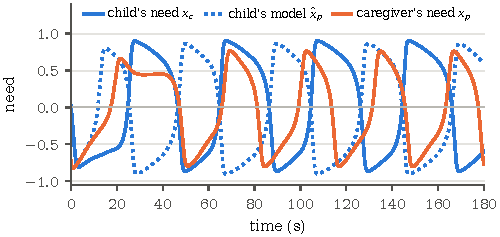
\includegraphics[width=\columnwidth]{figures/fig_belief_log.pdf}
\caption{Belief without coordination: controller logs of a Gazebo run with private models at $\eam=0.2$. The child's need and its model of the caregiver are in anti-phase, while the caregiver's need runs at a different frequency.}
\label{fig:belief}
\end{figure}

\subsection{The identical-start illusion}
\label{sec:r3}
From identical starting needs, private models under avoidance stay perfectly synchronised, offline (dashed line in Fig.~\ref{fig:strips}a) and on the robots (open markers). The symmetric start keeps the two halves of every copy equal, so the robots' estimates coincide, but this state is unstable (Fig.~\ref{fig:stability}). A difference of $10^{-7}$ in the starting accumulated needs separates the robots' needs after 704~s at $\eav=0.1$ and 421~s at $\eav=0.2$, and a difference of 0.1 within 18~s. Each hundred-fold reduction delays the separation by about 190~s at $\eav=0.1$, the signature of exponential growth, and over the last 330~s of a 2000~s run the coordination lies within 0.1 of zero, whereas the coupled reference returns to synchrony. On the robots the symmetric state persisted, because blind estimates make the needs independent of behaviour; any perturbation, from noisy perception or an asymmetric start, would end it. Robot studies of coupled dynamics are often run from one convenient start; here that would have suggested that private models preserve avoidant synchrony. Pulse-coupled oscillators synchronise from almost all starting states~\cite{Mirollo1990}; this dyad from almost none.

\begin{figure}[t]
\centering
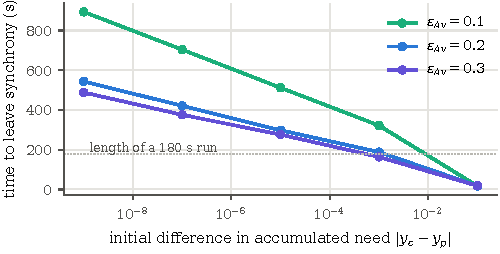
\includegraphics[width=\columnwidth]{figures/fig_stability.pdf}
\caption{The identical start is unstable. Private models under avoidance, started from identical needs with the caregiver's accumulated need raised by a small amount: time until the robots' needs first differ by more than 0.1.}
\label{fig:stability}
\end{figure}

\subsection{Anchoring restores coordination}
\label{sec:r4}
Under ambivalence, where every design stays bounded for $0.1\leq\eam\leq0.4$, only the anchored design restores coordination (Fig.~\ref{fig:anchoring}). Its partner model tracks the caregiver with a correlation of $0.76\pm0.11$, against 0.13--0.31 in the other private designs, and the robots' needs anti-synchronise again, at $-0.62\pm0.14$ against $-0.06$ to $-0.20$; the coupled reference, at $-0.93$, remains tighter. The anchored caregiver answers 0.35 of the child's calls, close to the reference's 0.25. Under avoidance only $\eav=0.1$ keeps every design bounded; there the anchored partner model tracks the caregiver at 0.79, and the needs synchronise at 0.60 against 0.79 for the reference.

\begin{figure*}[t]
\centering
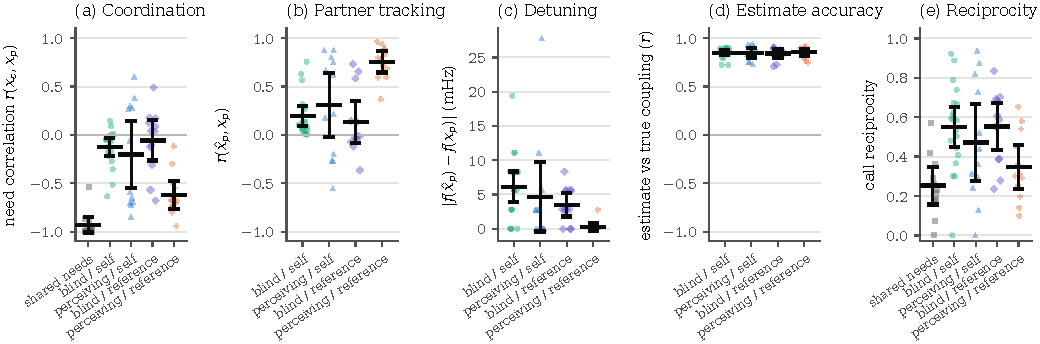
\includegraphics[width=\textwidth]{figures/fig_anchoring.pdf}
\caption{Anchoring restores coordination. Gazebo runs under ambivalence, pooled over $0.1\leq\eam\leq0.4$ (random starts, runs that escaped omitted), for the coupled reference (``shared needs'') and the four private designs, named by perception and partner model. Points: runs; bars: mean and 95\% interval. (a) Coordination. (b) Partner tracking. (c) Detuning between the child's model of the caregiver and the caregiver's need. (d) Accuracy of the child's estimate. (e) Call reciprocity.}
\label{fig:anchoring}
\end{figure*}

Why does anchoring work? Not because the anchored robot estimates better: the child's estimate follows the coupling terms of the true needs equally well in all four designs, at correlations near 0.85 (Fig.~\ref{fig:anchoring}d). The difference lies in the detuning. The anchored partner model runs within 0.2~mHz of the caregiver's need, against 3.5--6.1~mHz in the other designs (Fig.~\ref{fig:anchoring}c), and the child's own need runs 1.6~mHz from the caregiver's, against 3.7--5.6~mHz. We read this as a chain of entrainment: perception ties the child's need to the real caregiver, and the reference model ties the partner model to the child's need, as in the coupled model. Remove either link and the robots stay detuned. The estimate itself needs perception under avoidance, where it follows the true coupling at 0.97 with heard calls and is inverted, at $-0.51$ to $-0.80$, with silent ones; the caregiver's estimate is poor in every design (Section~S5). Anchoring also costs stability: the anchored dyad escapes from $\eam=0.6$ and $\eav=0.2$.

\subsection{Reading attachment from behaviour}
\label{sec:r5}
The regimes leave a mark in behaviour that an observer can read. Over 15 minutes the reference caregiver keeps its pattern of responses, while with private models reciprocity wanders between 0.18 and 1.00 (Section~S6). Observers trained only on the kinematic stand-in classified the regime of 60\% of 176 Gazebo runs from the child's behaviour, where chance is one in three, and 89\% from both robots', equally from identical and random starts (Table~\ref{tab:inverse}); the parameter error fell from 0.18--0.19 to 0.05--0.07. The caregiver's calls carried half of the information. A robot could thus estimate the relational parameters its networks now take as inputs, and the result echoes the link between maternal responsiveness and infant pattern~\cite{Ainsworth1978} and the objective SSP measures of~\cite{Prince2021}.

\begin{table}[t]
\centering
\caption{Reading the attachment parameters from behaviour. Stand-in CV: five-fold cross-validation by seed on the stand-in; Gazebo transfer: trained on the stand-in, tested on the 176 Gazebo runs; Gazebo CV: within the Gazebo runs, folds by seed.}
\label{tab:inverse}
\footnotesize
\setlength{\tabcolsep}{3pt}
\resizebox{\columnwidth}{!}{\begin{tabular}{@{}lrrrrr@{}}
\toprule
Observer & Stand-in CV & Gazebo transfer & Gazebo CV & MAE $\varepsilon_{Av}$ & MAE $\varepsilon_{Am}$ \\
\midrule
Child only & 65\% & 60\% (106/176) & 56\% & 0.18 & 0.19 \\
Both agents & 85\% & 89\% (156/176) & 74\% & 0.05 & 0.07 \\
\bottomrule
\end{tabular}
}
\end{table}

% =====================================================================
\section{Discussion}
\label{sec:discussion}

\subsection{Grounding the coupling of interacting robots}
The coupled model of Section~\ref{sec:model} has a rich repertoire, and Section~\ref{sec:behaviour} shows that its regimes are visible in distance and calls, in simulation and on physical robots. That is what makes grounding possible: a robot can learn the coupling terms from what it senses. It is not what makes grounding work. The four estimation-coupled designs estimate the coupling equally well, and only the anchored one coordinates. The failure mode, detuning between partners' internal rhythms, is generic to coupled oscillators~\cite{Kelso1995,Ermentrout2019}, so the lesson should hold for any robot whose internal rhythm is meant to resonate with a partner's~\cite{Lomas2022resonance}. The anchored design anchors indirectly, through the robot's own need. A more direct route is to correct the partner model with the partner's observed behaviour, for instance by resetting its phase at each call as pulse-coupled oscillators do~\cite{Mirollo1990}, or with an observer for coupled oscillators \citeneeded{state estimation / observers for coupled oscillators}. For method, symmetric starts can sit on invariant but unstable sets, so robot studies should vary them, and validating every run against its controller separates what the robots express from what they cause.

\subsection{What the model says about attachment}
The coupled model maps the attachment dimensions onto distinct dynamics: synchrony for a secure dyad, anti-synchrony and an inhomogeneous steady state for an unavailable caregiver, a shared exploratory state for avoidance, and irregular oscillation near the transitions, a candidate for disorganisation~\cite{Gagliardi2021our}. The estimation-coupled robots add a reading of Bowlby's working models: the regimes belong to partners whose models of each other are fitted~\cite{Bowlby1982}, and unfitted models produce a dyad in which each partner represents a relationship that is not being enacted. This yields a testable prediction. In joint recordings of both partners in the SSP~\cite{Prince2021,Chow2018representing}, poorly fitted dyads should show individual rhythms more regular than their relative phase, so that biobehavioural synchrony~\cite{Feldman2017} would index the fit of the partners' models. Fitting is developmental, whereas our parameters and networks are fixed; letting them adapt~\cite{Thelen1994,Stevens2009dynamic,Wilson2021} is the next step.

\subsection{Limitations and ethics}
The estimation-coupled robots are simulated, with a Boolean stand-in for calls; the physical robots of Section~\ref{sec:behaviour} ran the coupled model. The robot controllers use the distance form, Eq.~\eqref{eq:distance}, whose oscillatory regimes match the coupled model's phase relations but which escapes where the model settles, and the networks were trained in a simulator with different dynamics and timescale from the controllers'. The anchoring result rests on 12 to 20 robot runs per design. We have not modelled development or interaction with people. A robot that reads a person's relational style could serve the person better or cultivate dependence~\cite{Sharkey2010,Prescott2021}; our results add that a robot whose partner model is not anchored to perception will act on a relationship that is not taking place, and its own model will not tell it so.

% =====================================================================
\section{Conclusion}
A coupled-oscillator model of attachment produces synchrony, anti-synchrony, steady states and irregular oscillation that correspond to attachment patterns, and these regimes are visible in distance and vocal exchange. Coupling two robots through estimates of the coupling terms, learned from those signals, grounds the model in perception, but only an anchored partner model, driven by a reference model while the robot perceives its partner, keeps the robots coordinated; private models detune, and their synchrony from identical starts is an illusion. For social robots, coupling must be grounded and anchored; for attachment, coordination is a joint achievement of working models fitted to each other.

\section*{Acknowledgements}
This work was supported by UK Research and Innovation (UKRI) under the UK government's Horizon Europe funding guarantee for the Horizon Europe EIC Pathfinder CAVAA project. AJR and AH are also supported by Innovate UK (grant number 10089807) for the European Union's Horizon Europe research and innovation programme under Grant Agreement no.~101120727 (PRIMI). \authornote{check that the funding statement is current}

\section*{Declaration of interest}
TJP is a director and shareholder of Consequential Robotics Ltd, which develops the MiRo robot, and of Bettering Our Worlds (BOW) Ltd, which develops robot software. The other authors have no competing interests.

\section*{Data and code availability}
The controllers, recorded runs and the scripts that produce every figure and number are available at \authornote{repository URL}.

\bibliographystyle{IEEEtran}
\bibliography{refs}

% ---------------------------------------------------------------- biographies
% Placeholders that reserve the space of the final biographies (about 100 words and a photo each),
% so that the page count of the draft matches the final paper. Replace before submission.
\newcommand{\bioplaceholder}{\textcolor{gray}{Placeholder for the biography (about 100 words): degrees with institutions and years, current position, research interests and professional memberships. This paragraph only reserves the space that the final biography will take, so that the page count of the draft matches the final paper. Replace it, and the photo frame, before submission; the text should state the author's research focus and any IEEE membership grade.}}
\begin{IEEEbiography}[\photoplaceholder]{Aung Htet}
\bioplaceholder
\end{IEEEbiography}
\begin{IEEEbiography}[\photoplaceholder]{Alejandro Jimenez-Rodriguez}
\bioplaceholder
\end{IEEEbiography}
\begin{IEEEbiography}[\photoplaceholder]{Marcantonio Gagliardi}
\bioplaceholder
\end{IEEEbiography}
\begin{IEEEbiography}[\photoplaceholder]{Tony J. Prescott}
\bioplaceholder\label{paper:end}
\end{IEEEbiography}

% ---------------------------------------------------------------- draft only (not part of the paper)
\ifdraftmarkers
\clearpage
\onecolumn
\section*{Draft only: citations to be sourced}
The following placeholders mark claims that need a reference beyond the reference lists of~\cite{Htet2024} and of the npj draft. This page is not part of the paper and disappears with \texttt{\textbackslash draftmarkersfalse}.
\listofcitationsneeded
\fi

\end{document}
